\section{Durchführung}
\label{sec:durchfuehrung}

    Der folgende Abschnitt beinhaltet die Durchführung der verschiedenen Messungen.

\subsection{Messung einer Entladekurve des Kondensators}

    Für die Bestimmung der Zeitkonstante $RC$ kann entweder die Entlade- oder die Aufladekurve des Kondensators untersucht werden.
    Hier wird die Entladekurve gemessen,
    wobei die verwendete Schaltung in der folgenden Abbildung \ref{fig:messung_entladekurve} dargestellt ist.

    \begin{figure}
        \centering
        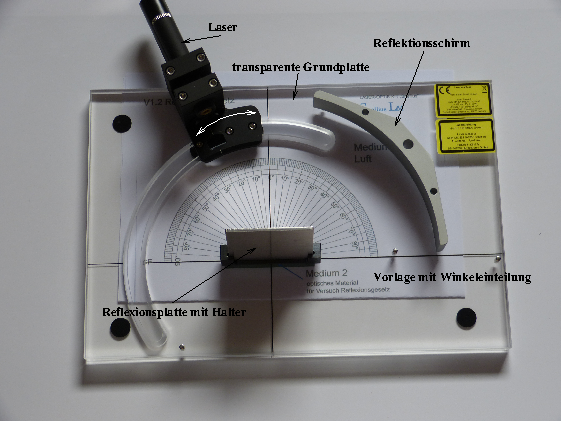
\includegraphics{content/img/Abb_3.pdf}
        \caption{Schaltung zur Messung der Auf- und Entaldekurve des Kondensators im RC-Kreis.}
        \label{fig:messung_entladekurve}
    \end{figure}

    Zu Beginn der Messung muss an Generator eine Rechteckspannung eingestellt werden,
    welche auf einem Oszilloskop in Abhängigkeit von der Zeit darstellbar ist.
    Die Entladekurve ist in Abbildung \ref{fig:entladekurve} zu sehen.

    \begin{figure}
        \centering
        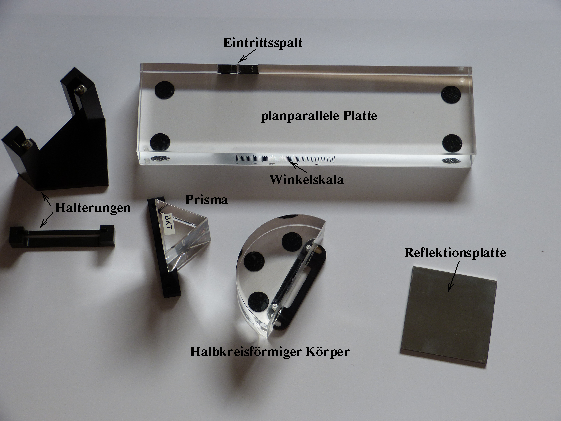
\includegraphics{content/img/Abb_4.pdf}
        \caption{Gestalt der Entladekurve.}
        \label{fig:entladekurve}
    \end{figure}

    Es werden fünfzehn Messwerte aufgenommen,
    wobei die Zeitkonstante mithilfe der Gleichung \eqref{eqn:entladung} berechnet werden kann.

\subsection{Messung der Amplitude und der Phasenverschiebung}

    Für diese Messung wird am Generator eine Sinusförmige Spannung angelegt,
    welche wieder auf einem Oszilloskop dargestellt werden kann.\\
    Für die Messung der Amplitude wird die folgende Schaltung verwendet.

    \begin{figure}
        \centering
        \includegraphics{content/img/Abb_5.pdf}
        \caption{Schaltung zur Messung der Spannungsamplitude in Abhängigkeit der Frequenz.}
        \label{fig:messung_amplitude}
    \end{figure}

    Zu Beginn wird die Frequenz der kleinst- und größtmöglich darstellbaren Amplitude bestimmt,
    in diesem Fall lag die größtmögliche Amplitude bei $\omega = \SI{10}{\hertz}$ und die kleinstmögliche Amplitude bei $\omega = \SI{2000}{\hertz}$.
    Anschließend wird das Intervall zwischen beiden Frequenzwerten in geeigneten Abständen ausgemessen.
    Die Zeitkonstante kann mit Umstellen der Gleichung \eqref{eqn:amplitude} berechnet werden.\\
    \\
    Die Messung der Phasenverschiebung kann mit denselben Einstellungen durchgeführt werden.

    \begin{figure}
        \centering
        \includegraphics{content/img/Abb_6.pdf}
        \caption{Schaltung zur Messung der Phasenverschiebung von Generatr- und Kondensatorspannung.}
        \label{fig:messung_phasenverschiebung}
    \end{figure}

    In Abbildung \ref{fig:messung_phasenverschiebung} ist die verwendete Schaltung gezeigt.
    Die Generatorspannung $U_\text{G}$ wird am Eingang $Y_\text{A}$ angeschlossen,
    die Kondensatorspannung $U_\text{C}$ am Eingang $Y_\text{B}$.
    Am Oszilloskop muss die Einstellung \textit{DUAL} ausgewählt werden,
    um gleichzeitig die eingehende Generatorspannung und die Kondensatorspannung zu sehen.
    Es wird dasselbe Frequenzintervall wie vorher abgelaufen,
    wobei die Abstände $a$ und $b$ entsprechend der Darstellung in Abbildung \ref{fig:phasenverschiebung} gemessen werden.

    \begin{figure}
        \centering
        \includegraphics{content/img/Abb_7_edit.pdf}
        \caption{Die Phasenverschiebung zwischen Generatorspannung und Kondensatorspannung.}
        \label{fig:phasenverschiebung}
    \end{figure}

    Die Phasenverschiebung kann mithilfe von
    \begin{align*}
        \phi &= \frac{a}{b} \cdot 360 & \phi &= \frac{a}{b} \cdot 2 \symup{\pi}
    \end{align*}
    bestimmt und in Gleichung \eqref{eqn:phasenverschiebung} zur Berechnung der Zeitkonstante eingesetzt werden.
